
%% ----------------------------------------------------------------
%% Thesis.tex -- MAIN FILE (the one that you compile with LaTeX)
%% ---------------------------------------------------------------- 

% Set up the document
\documentclass[a4paper, 10.5pt, twosided, hidelinks]{Thesis}  % Use the "Thesis" style, based on the ECS Thesis style by Steve Gunn
\usepackage[italian, english]{babel}

% Figures
\usepackage{graphicx}
\graphicspath{{Figures/}}  % Location of the graphics files (set up for graphics to be in PDF format)


% Hyperref
\usepackage{hyperref}
\usepackage[dvipsnames]{xcolor}
 \usepackage{breakurl}
\hypersetup{
	pdfauthor  = {name},
	pdfsubject = {PhD thesis},
	pdftitle   = {PhD thesis},
	pdfcreator = {name}
} 


% Bibliography
\usepackage{natbib}
%\bibliographystyle{apa}


\usepackage{amsfonts, amsmath, amssymb, bm}
\usepackage{amsthm}


% Page style
\usepackage{fancyhdr}
\let\Sectionmark\sectionmark
\def\sectionmark#1{\def\Sectionname{#1}\Sectionmark{#1}}
\usepackage{tgpagella}%tgpagella palatino

%\usepackage{verbatim}  % Needed for the "comment" environment to make LaTeX comments
%\usepackage{bigints}
%\usepackage[autostyle]{csquotes}  
%\usepackage{psfrag}
%\usepackage{tikz}
%\usetikzlibrary{fit,positioning,calc}
%\usepackage{colortbl}
%\usepackage{dashrule}
%\usepackage{booktabs}
%\usepackage{url}
%\usepackage{color, caption, multirow}
%\usepackage{indentfirst}
%\usepackage{multirow}
%\usepackage{lipsum}
%\usepackage{algorithm}
%\usepackage{algorithmic}
%\usepackage{float}

\usepackage[titletoc,title]{appendix}
\usepackage{pdfpages}

%%% TITLE
\renewcommand{\maketitle}{
\begin{titlepage}%
	\thispagestyle{empty} \enlargethispage{18cm} \noindent
	\begin{figure}
		\centering
\includegraphics{Figures/logo}
	\end{figure}
	\begin{flushleft}
		Sede Amministrativa: Universit\`a degli Studi di Padova
	\end{flushleft}
	\begin{flushleft}
		\vspace{1cm}
		Dipartimento di Scienze Statistiche\\
		Corso di Dottorato di Ricerca in Scienze Statistiche\\
		Ciclo XXXIV
	\end{flushleft}
	\vspace{1cm}
	
	\begin{center}
		\LARGE\textbf{Thesis Title}
	\end{center}
	
	\begin{flushleft}
		\vspace{1.5cm}
		\textbf{Coordinatore del Corso:} Prof. Nicola Sartori\\
		\vspace{0.5cm}
		\textbf{Supervisore:} Prof. Antonio Canale\\
		\vspace{0.5cm}
		\textbf{Co-supervisore:} Prof. Michele Guindani\\
	\end{flushleft}
	
	\begin{flushright}
		\vspace{2cm}
		\textbf{Dottoranda:} Laura D'Angelo
	\end{flushright}
	\begin{flushleft}
		\vspace{1cm}
		Day Month Year of submission
	\end{flushleft}
\end{titlepage}
}
\makeindex  







%%----------------------------------------------------------------
\begin{document}
\maketitle

\frontmatter	  % Begin Roman style (i, ii, iii, iv...) page numbering

\setcounter{page}{1}
\pagenumbering{roman}
%%----------------------------------------------------------------

\setstretch{1.3}  % It is better to have smaller font and larger line spacing than the other way round
\setlength{\parindent}{3ex}
\fancyhead{}  
\rhead{\thepage} 
\lhead{}  

\pagestyle{empty}  
\cleardoublepage

\setstretch{1.3}  
\pagestyle{empty} 


%%----------------------------------------------------------------

%%%%%%%%%%%%%%%%%%%%%%% Absract %%%%%%%%%%%%%%%%%%%%%%%%%

\btypeout{Abstract Page}
  \null\vspace{4cm}
  \begin{center}
	  \setlength{\parskip}{0pt}
	  {\huge{{\textbf{Abstract}}} \par}
	  \bigskip
  \end{center}
Abstract content.


\pagestyle{empty}  % Page style needs to be empty for this page
\cleardoublepage
\pagestyle{plain}
%% ----------------------------------------------------------------

\newpage
\thispagestyle{empty}
\mbox{}

%%%%%%%%%%%%%%%%%%%%%%% Put Sommario here %%%%%%%%%%%%%%%%%%%%%%%%%

\pagestyle{empty}
\btypeout{Abstract Page}
  \null\vspace{3cm}
\begin{center}
   \setlength{\parskip}{0pt}
   {\huge{{\textbf{Sommario}}} \par}
   \bigskip
\end{center}
\selectlanguage{italian}
Contenuto del sommario.


\selectlanguage{english}

% Sommario ended, start a new page
\newpage
\thispagestyle{empty}
\mbox{}


%-------------------------- Dedica --------------------------%
%\newpage
%\thispagestyle{empty}
%\mbox{}
%
%\topskip0pt
%\vspace*{4cm}
%\begin{flushright}
%	\textit{\Large{{Dedication}}}
%\end{flushright}
%\vspace*{\fill}
%\newpage
%\thispagestyle{empty}
%\mbox{}

%------------------------------------------------------------%
%-------------------------- Acknowledgements --------------------------%
%\newpage
%\thispagestyle{empty}
%\mbox{}
%
%\thispagestyle{empty}
%\btypeout{Abstract Page}
%
%\begin{center}
%    \setlength{\parskip}{0pt}
%    {\huge{\textbf{Acknowledgements}} \par}
%        \bigskip
%\end{center}
%{ Acknowledgements content.}
%
%
%\newpage
%\thispagestyle{empty}
%\mbox{}
%------------------------------------------------------------%

\fancyhead[LE]{\thepage}
\fancyhead[RE]{Contents}

\pagestyle{fancy}  %The page style headers have been "empty" all this time, now use the "fancy" headers as defined before to bring them back

\tableofcontents  % Write out the Table of Contents
\newpage
\thispagestyle{empty}
\mbox{}

%%----------------------------------------------------------------



 \cleardoublepage\phantomsection
 \fancyhead[RO,LE]{\thepage}
 \fancyhead[RE]{List of Figures}
 \fancyhead[LO]{List of Figures}
 \pagestyle{fancy}

\listoffigures  % Write out the List of Figures
\clearpage
\pagestyle{empty}
%%----------------------------------------------------------------


\clearpage\phantomsection
\fancyhead[RO,LE]{\thepage}
\fancyhead[RE]{List of Tables}
\fancyhead[LO]{List of Tables}
\pagestyle{fancy}

\listoftables  % Write out the List of Tables

\clearpage\phantomsection
\pagestyle{empty}


%%----------------------------------------------------------------
\addtocontents{toc}{\vspace{1em}}
  % Return the page headers back to the "fancy" style
\mainmatter	  % Begin normal, numeric (1,2,3...) page numbering

% Include the chapters of the thesis, as separate files
% Just uncomment the lines as you write the chapters
\cleardoublepage\phantomsection
\pagestyle{fancy}
% Introduction
\addcontentsline{toc}{chapter}{Introduction}
\chapter*{Introduction} % Write in your own chapter title



\fancyhead[RO,LE]{\thepage}
\fancyhead[LO]{\emph{Introduction}}
\fancyhead[RE]{\emph{Overview}}

\setlength{\parskip}{0.5pt}

\bigskip

\addcontentsline{toc}{section}{Overview}
\section*{Overview}

A fundamental but unsolved problem in neuroscience is understanding the functioning of neurons and neuronal networks in processing sensory information, generating locomotion, and mediating learning and memory.
The investigation of the structure and function of the nervous system can be dated back to the nineteenth century with the invention of the technique of silver impregnation by Camillo Golgi in 1873, which allowed the visualization of individual neurons~\citep{drouin2015}. The technique initiated the study of the microscopic anatomy of the nervous system, and the investigation of how neurons organize to form the brain. 
Ever since there has been a significant research effort both to discover the cellular properties of the nervous system, and to characterize behaviors and correlate them with activity imaged in different regions of the brain.
However, many scientists recognize that despite the innovative techniques developed to observe and analyze neurons, we are still facing an ``explanatory gap'' between the understanding of elemental components and the outputs that they produce~\citep{parker2006,parker2010,dudai2004}. That is, we know a lot about the components of the nervous system, but still we have little insight into how these components work together to enable us to think, remember, or behave. One of the reasons of this gap is the availability of a huge quantity of data, but a lack of tools to integrate these data in order to obtain a coherent picture of the brain functioning~\citep{parker2010}.

The technological developments of the last few decades have opened fundamentally new opportunities to investigate the nervous system. Large neuronal networks can now be visualized using \textit{in vivo} high-resolution imaging techniques, which permit to record the neuronal activity in freely moving animals over long periods of time. In this thesis, we focus on data resulting from the application of the two-photon calcium imaging technique. Calcium ions generate intracellular signals that determine a large variety of functions in all neurons: when a neuron fires, calcium floods the cell and produces a transient spike in its concentration~\citep{grienberger2012}. By using genetically encoded calcium indicators, which are fluorescent molecules that react when binding to the calcium ions, it is possible to optically measure the level of calcium by analyzing the observed fluorescence trace. 
However, extracting these fluorescent calcium traces is just the first step towards the understanding of brain circuits: how to relate the observed pattern of neuronal activity with its output remains an open problem of research.



\phantomsection
\addcontentsline{toc}{section}{Main contributions of the thesis}
\fancyhead[RE]{\emph{Main contributions of the thesis}}
\section*{Main contributions of the thesis}


\noindent

 

% Chapter 1
\chapter{Background: statistical modeling of calcium imaging data}
\fancyhead[RO,LE]{\thepage}
\fancyhead[LO]{Chapter 1 - \emph{Background}}
\fancyhead[RE]{Section \thesection \ - \emph{\Sectionname}}

\setlength{\parskip}{0.5pt}

\bigskip

\section{Overview of calcium imaging data} 

Calcium ions generate intracellular signals that control key functions in all types of neurons.
At rest, most neurons have an intracellular calcium concentration of about 100 nm; however, during electrical activity, the concentration can rise transiently up to levels around 1000 nm~\citep{berridge2000}. 
The development of techniques that enable the visualization and quantitative estimation of the intracellular calcium signals have thus greatly enhanced the investigation of neuronal functioning.
The development of calcium imaging techniques involved two parallel processes: the development of calcium indicators, which are fluorescent molecules that react when binding to the calcium ions, and the implementation of the appropriate imaging instrumentation, in particular, the introduction of two-photon microscopy~\citep{denk1990}.
In recent years, the innovation achieved in these two fields has allowed for real-time observation of biological processes at the single-cell level simultaneously for large groups of neurons~\citep{grienberger2012}. 

The output two-photon calcium imaging is a movie of time-varying fluorescence intensities, and a first complex pre-processing phase deals with the identification of the spatial location of each neuron in the optical field and source extraction~\citep{mukamel2009,dombeck2010}. The resulting processed data consist of a fluorescent calcium trace for each observable neuron in the targeted area which, however, is only a proxy of the underlying neuronal activity.
Hence further analyses are needed to deconvolve the fluorescence trace to extract the spike train (i.e. the series of recorded firing times), and to try to explain how these firing events are linked with the experiment that generated that particular pattern of activity.

\subsection{Deconvolution methods}

There is currently a rich literature of methods addressing the issue of deconvolving the raw fluorescent trace to extract the spike train. A successful approach is to assume a biophysical model to relate the spiking activity to the calcium dynamics, and to the observed fluorescence. \citet{vogelstein2010} proposed a simple but effective model that has later been adopted by several authors~\citep{pnevmatikakis2016, friedrich2016, friedrich2017, jewell2018, jewell2019}. The model considers the observed fluorescence as a linear (and noisy) function of the intracellular calcium concentration; the calcium dynamics is then modeled using an autoregressive process with jumps in correspondence of the neuron's firing events.
Denoting with $y_t$ the observed fluorescence trace of a neuron and with $c_t$ the underlying calcium concentration, for time $t=1,\dots,T$, the model can be written as
\begin{equation}
\begin{gathered}
y_t = b + c_t + \epsilon_t,\quad \epsilon_t \sim \N(0,\sigma^2),  \\
c_t = \gamma\, c_{t-1} + A_t + w_t, \quad w_t \sim \N(0, \tau^2),
\end{gathered}
\label{eq:ch1_armodel}
\end{equation}
where $b$ models the baseline level of the observed trace and $\epsilon_t$ is a Gaussian measurement error. In the absence of neuronal activity, the true calcium concentration $c_t$ is considered to be centered around zero. The parameter $A_t$ captures the neuronal activity: in the absence of a spike ($A_t = 0$), the calcium level follows a AR(1) process controlled by the parameter $\gamma$; when a spike occurs, the concentration increases instantaneously of a value $A_t > 0$.
A challenge remains estimating the neuronal activity $A_t$ in a precise and computationally efficient way.

\citet{vogelstein2010} assume that all spikes have a fixed amplitude, and interpret the parameter $A_t$ as the \textit{number} of spikes at time $t$. Following this definition, they place a Poisson prior distribution on $A_t$; however, the maximum a posteriori estimation of the spike train using a Poisson distribution is computationally intractable. Hence they search an approximate solution by replacing the Poisson distribution with an exponential distribution of the same mean. This leads to some loss of interpretation of the parameters $A_t$, as now they are no longer integer values but rather non-negative real numbers, but turns the problem into a convex optimization, which can be solved efficiently.
Adopting this approach leads to solving a non-negative lasso problem for estimating the calcium concentration, where the $L_1$ penalty enforces sparsity of the neural activity.
Efficient algorithms to obtain a solution of this problem were also proposed by \citet{pnevmatikakis2016}, \citet{friedrich2016}, and \citet{friedrich2017}.

A different perspective is instead proposed by~\citet{jewell2018} and~\citet{jewell2019}: rather than interpreting $A_t$ in model~(\ref{eq:ch1_armodel}) as the number of spikes at the $t$-th timestep, they interpret its sign as an indicator for whether or not \textit{at least one} spike occurred, that is, $A_t = 0$ indicates no spikes at time $t$, and $A_t>0$ indicates the occurrence of at least one spike. The model so formulated includes an indicator variable, which corresponds to using an $L_0$ penalization and which makes the optimization problem highly non-convex. 
In their work, \citet{jewell2018} and~\citet{jewell2019} develop fast algorithms to compute the spike trains under these assumptions.
\citet{jewell2018} assert that the solutions discussed by \citet{vogelstein2010}, \citet{friedrich2016}, and \citet{friedrich2017} can actually be seen as convex relaxations of this optimization problem, to overcome the computational intractability of the $L_0$ penalization. 

Finally,~\citet{pnevmatikakis2013} propose a fully Bayesian approach. Although less computationally efficient than optimization methods, it allows to obtain a posterior distribution of all model parameters instead of just a point estimate, hence improving uncertainty quantification.
Differently from previous models, they define the parameter $A_t$ as the \textit{amplitude} of a spike at time $t$, taking values in the non-negative real numbers.
They formulate the presence/absence of a spike and its amplitude by using the product of a Bernoulli random variable (taking value 0 if there is no spike at time $t$, and 1 otherwise) with a half-Gaussian random variable (modeling the positive amplitudes). However, they do not explicitly assume sparsity of the spikes.

\section{Data sets} 
Una frase introduttiva? Parlo dei dati dell'Allen Brain Observatory e poi ci sarebbe da mettere i nuovi dati se riesco a fare qualcosa del progetto 3...

\subsection{Allen Brain Observatory data}
The Allen Brain Observatory~\citep{allen} is a public large data repository for investigating how sensory stimulation is represented by neural activity in the mouse visual cortex in both single cells and populations.
The project aims to provide a standardized and systematic survey to measure and analyze visual responses from neurons across cortical areas and layers, utilizing transgenic Cre lines to drive expression of genetically encoded fluorescent calcium indicators, and measured by \textit{in vivo} two-photon calcium imaging.

The study is an extended survey of physiological activity in the mouse visual cortex in response to a range of visual stimuli~\citep{allen_stimulus}. Each mouse is placed in front of a screen where different types of visual stimuli are shown, while the mouse’s neuronal activity is recorded. The stimuli vary from simple synthetic images such as locally sparse noise or static gratings, to complex natural scenes and movies.
The goal of the study is to investigate how neurons at different depths in the visual areas respond to stimuli of different complexity. Specifically, each neuron in the visual cortex can be characterized by their \textit{receptive field}, i.e. the features of the visual stimulus that trigger the signaling of that neuron. Hence, it is of critical interest to devise methods that allow inferring how the neuronal response varies under the different types of visual stimuli. %We expect that the neuronal activity will vary across all the experimental settings, and that some variations in its intensity will be observed based on the specific visual stimulus.


\subsection{Altri dati?}
Paragrafo qui.

\section{A brief review of some Bayesian nonparametric models} 
In this section we review some statistical tools that will be employed in this thesis in the analysis of calcium imaging data. The purpose of this section is not to provide a comprehensive review, but rather to outline the theoretical framework we adopted and fix some notation.
The core topic will be the Bayesian methodology, with a focus on Bayesian nonparametric models.

\subsection{Finite mixture models}
\label{subsec:finite_mix}
We start our discussion by reviewing finite mixtures. Although they are not part of the Bayesian nonparametric methodology, they provide the starting point for many models that we will review in the following. The content of this brief overview on finite mixtures is largely based on the dedicated chapter in~\citet{gelman2013}.

\subsubsection*{Definition and hierarchical representations}
Mixtures are a popular tool to model heterogeneous data, characterized by the presence of subpopulations within the overall population. In many practical problems the data are collected under different conditions -- unfortunately, it is not always possible to have information on the subpopulation to which each individual observation belongs.
Mixture models can be used in problems of this type, where the population consists of a number of latent subpopulations, within each of which a relatively simple model can be applied.

Denote the observed data as a vector of $n$ units $\bm{y} = (y_1,\dots,y_n)$; also, assume that the $n$ observations are exchangeable, meaning that the joint probability density $p(y_1,\dots,y_n)$ is invariant to permutations of the indices. In the framework of finite mixtures, we assume that the population is made of $K\leq n$ subpopulations, with $K$ known and fixed.
We assume that within each of these groups, the distribution of $y_i$, $i=1,\dots,n$, can be modeled as $f(y_i \mid \theta_k^*)$, for $k=1,\dots,K$. Usually a common parametric family is assumed for all these component distributions, which however depend on specific parameter vectors $\theta_k^*$.
The last missing piece to construct a mixture model is the parameter describing the proportion of population from each component $k$: we denote this parameter with $\pi_k$, satisfying $\sum_{k=1}^K \pi_k = 1$. Denoting the full vectors of parameters as $\bm{\theta}^* = (\theta_1^*,\dots,\theta_K^*)$ and $\bm{\pi} = (\pi_1,\dots,\pi_K)$, the data distribution for observation $i$ can be formulated as
\begin{equation*}
p(y_i\mid \bm{\theta}^*,\bm{\pi}) = \pi_1 \, f(y_i\mid\theta_1^*) + \dots + \pi_K \, f(y_i\mid\theta_K^*).
\end{equation*}

In mixture models it is convenient to think of the component indicators as missing data, and to impute them to obtain a much simpler form of the data distribution. Hence we introduce the indicator $S_{ik}$ of component $k$ for observation $i$, with 
\begin{equation*}
S_{ik} = \begin{cases}
1 \quad \text{if $y_i$ is drawn from component $k$}\\
0 \quad \text{otherwise}.
\end{cases}
\end{equation*}
Given $\bm{\pi}$, the distribution of $\bm{S}_i = (S_{i1},\dots,S_{iK})$ is $\Mult(1;\pi_1,\dots,\pi_K)$. 
Conditionally on $\bm{S}_{i}$, the data distribution of $y_i$ is simply $p(y_i\mid \bm{S}_i,\bm{\theta}^*) = \prod_{k=1}^K f(y_i\mid\theta_k^*)^{S_{ik}}$; moreover, given $\bm{S}=(\bm{S}_1,\dots,\bm{S}_n)$, the $y_i$ are assumed to be independent.
The joint density of the observed data and the unobserved indicators, conditionally on the model parameters, can now be written as 
\begin{equation*}
p(\bm{y},\bm{S}\mid \bm{\theta}^*,\bm{\pi}) = p(\bm{y}\mid\bm{S},\bm{\theta}^*)\, p(\bm{S}\mid\bm{\pi}) = 
\prod_{i=1}^n \prod_{k=1}^K \left\{ \pi_k f(y_i\mid\theta_k^*) \right\}^{S_{ik}}.
\end{equation*}

Having defined the data distribution, we need to specify adequate prior distributions on the model parameters $\bm{\pi}$ and $\bm{\theta}^*$. The prior $G_0$ on $\bm{\theta}^*$ is usually chosen depending on the specific application and on the basis of the component distribution $f$. For the mixture proportions $\pi_k$, the conjugate and most natural prior distribution is the Dirichlet distribution, $\bm{\pi}\sim \Dir_K(\alpha_1,\dots,\alpha_K)$.

This model also admits a useful hierarchical representation. Rewriting the latent allocation variables using the cluster indicators $c_i\in\{1,\dots,K\}$, with $c_i=k$ if $y_i$ belongs to the $k$-th mixture component (i.e. $S_{ik} = 1$), the model is, for $i = 1,\dots,n$ 
\begin{equation}
\begin{gathered}
\pi_1,\dots,\pi_K  \sim \Dir_K(\alpha_1,\dots,\alpha_K)\\
\theta^*_1,\dots,\theta^*_K \sim G_0\\
\Pr(c_i = k \mid \pi_1,\dots,\pi_K) = \pi_k \quad \text{for } k = 1,\dots,K\\ 
y_i \mid c_i = k, \theta^*_k \sim f(y_i\mid\theta^*_k).
\end{gathered}
\label{eq:ch1_finitemix_h1}
\end{equation}

It is possible to rewrite equation (\ref{eq:ch1_finitemix_h1}) in a slightly different way by thinking that each observation $y_i$ is associated with a parameter $\theta_i$, where these parameters are drawn from a discrete distribution $G$ with support on the $K$ locations $\{\theta^*_1,\dots,\theta^*_K\}$. The model then becomes, for $i=1,\dots,n$
\begin{equation}
\begin{gathered}
\pi_1,\dots,\pi_K \sim \Dir_K(\alpha_1,\dots,\alpha_K) \\
\theta^*_1,\dots,\theta^*_K \sim G_0\\
\theta_i \mid \bm{\theta}^*,\bm{\pi} \sim G = \sum_{k=1}^K \pi_k \delta_{\theta^*_k}\\
y_i \mid \theta_i \sim f(y_i\mid\theta_i).
\end{gathered}
\label{eq:ch1_finitemix_h2}
\end{equation}

\subsubsection*{Posterior inference for finite mixture models}
Posterior inference for mixture models is usually performed through Markov Chain Monte Carlo (MCMC) methods and, in particular, the Gibbs sampler, as the full conditionals after imputing the cluster indicators $\CC = \{c_1,\dots,c_n\}$ are greatly simplified.
Moreover, for the distribution of the mixture weights it is possible to exploit the conjugacy of the Dirichlet distribution with the multinomial model. A Gibbs sampler then simply iterates these three steps:
\begin{enumerate}
	\item Update the cluster-specific parameters $\theta^*_k$, for $k=1,\dots,K$, from
	$$ p(\theta^*_k \mid \CC, \bm{y}) \propto G_0(\theta^*_k) \prod_{i:c_i=k} f(y_i\mid\theta^*_{k}). $$
	\item Update the weights $\pi_1,\dots,\pi_K$ by sampling from a Dirichlet distribution with updated parameters
	$$ \pi_1,\dots,\pi_K\mid \CC \sim  \Dir_K(\alpha_1 + n_1,\dots,\alpha_K + n_K) $$
	where $n_k$ is the number of observations allocated to cluster $k$, for $k=1,\dots,K$.
	\item Update the cluster indicators: for $i=1,\dots,n$ and $k=1,\dots,K$,
	$$ \Pr(c_i = k\mid \bm{\pi},\bm{\theta}^*, y_i) \propto \pi_k f(y_i\mid\theta^*_{k})  .$$
\end{enumerate}

\subsection{Dirichlet process mixtures}
Nonparametric mixtures extend model (\ref{eq:ch1_finitemix_h2}) by placing a nonparametric prior on $G$. The most common prior on random probability measures is the Dirichlet process (DP), introduced by \citet{ferguson1973, ferguson1974}. Draws from a DP are discrete distributions with probability one, hence they turned out useful as flexible mixing measures in discrete mixtures.

\subsubsection*{The Dirichlet process }
A random distribution $G$ on $\Theta$ is said to follow a DP prior with base measure $G_0$ and concentration parameter $\alpha$, denoted $G\sim\DP(\alpha,G_0)$, if for any partition $\{B_1,\dots,B_H\}$ of $\Theta$, 
\begin{equation*}
(G(B_1),\dots,G(B_H)) \sim \Dir_H\big(\alpha G_0(B_1),\dots,\alpha G_0(B_H)\big).
\end{equation*}
The success of the DP mainly arises from two appealing characteristics: its large support, with respect to the space of probability distributions, and tractability of the posterior distribution.
%
Closely related to this last aspect is the conjugacy property of the DP: as the finite dimensional Dirichlet distribution is conjugate to the multinomial likelihood, the DP is conjugate with respect to i.i.d. sampling, that is, with respect to a completely unknown distribution from i.i.d. data.
More precisely, if we take $\{\theta_1,\dots,\theta_n\}$ a sequence of independent draws from $G\sim\DP(\alpha,G_0)$, then the posterior distribution of $G$ given these observed values is still a DP. 
Letting again $\{B_1,\dots,B_H\}$ be a finite measurable partition of $\Theta$, and letting $n_h$ be the number of observed values in $B_h$, for $h = 1,\dots,H$, the posterior distribution is given by
\begin{equation*}
(G(B_1),\dots,G(B_H))\mid \theta_1,\dots,\theta_n \sim \Dir_H\big(\alpha G_0(B_1) + n_1,\dots,\alpha G_0(B_H) + n_H\big).
\end{equation*}
In other terms, the posterior distribution is still DP with updated parameters:
\begin{equation*}
G \mid \theta_1,\dots,\theta_n \sim \DP \left(\alpha + n, \frac{\alpha G_0 + \sum_{i=1}^n \delta_{\theta_i}}{\alpha + n} \right).
\end{equation*}

The DP admits several nice representations. An intuitive constructive definition of a DP random probability measure is given by \citet{sethuraman1994} and is based on the discrete nature of the process, which can be represented as a a weighted sum of point masses. This definition states that if  $G\sim \DP(\alpha, G_0)$, then it can be expressed as follows:
\begin{equation*}
\begin{gathered}
\beta_k \sim \Beta(1,\alpha), \qquad \pi_k = \beta_k \prod_{l = 1}^{k-1} (1-\beta_l)\\
\theta^*_k \sim G_0, \qquad
G = \sum_{k=1}^{\infty} \pi_k \delta_{\theta^*_k}.
\end{gathered}
\end{equation*}

\subsubsection*{Dirichlet process mixtures}
Getting back to the framework of mixture models, from this representation it is straightforward to extend the finite mixtures described above to nonparametric mixtures: following the structure of equation (\ref{eq:ch1_finitemix_h2}), DP mixtures (DPM) can be written as
\begin{equation*}
\begin{gathered}
G \sim \DP(\alpha,G_0)\\
\theta_i \mid G \sim G \\
y_i \mid \theta_i \sim f(y_i\mid\theta_i).
\end{gathered}
\end{equation*}
Differently from the mixtures described in the previous section, DPM are an infinite mixture model, as they assume a countably infinite number of components. 
However, because the $\pi_k$'s decrease exponentially quickly, only a small number of components will be used to model the
data a priori: in the following, we will define \textit{clusters} these non-empty components. In general, the prior expected number of clusters, which corresponds to the number of distinct $\theta_i$ in a sample of $n$ values, is approximately equal to $\alpha \log(1 + n/\alpha)$.
This means that while in finite mixture models the number of clusters has to be fixed in advance, in DP mixture model, the number of clusters is determined by the data and can be inferred.

\subsubsection*{Posterior inference for DPM}


\subsection{Mixtures of finite mixtures}
To avoid fixing the number of clusters, a different approach to DP mixtures is to consider finite mixtures with a prior on the number of components. Although this may seem as the most natural way to infer the number of groups, application of mixtures of finite mixtures (MFM) has long been hindered by the difficulty of performing posterior inference. 
Several inference methods have been proposed for this type of model \citep{McCullagh2008,nobile2004,nobile2007,richardson1997} often exploiting the reversible jump Markov chain Monte Carlo technique. However, applying the reversible jump in new situations can be hard, as it requires designing new reversible jump moves.

More recently, different models have been proposed inspired by nonparametric mixtures. \citet{miller2018} explicitly derived MFM counterparts for several properties exhibited by DPM. They considered a finite mixture model similar to the one defined in section \ref{subsec:finite_mix}, where however the number of clusters is random and is assigned a prior distribution. A main limitation of their approach is that it is assumed a fixed parameter $\alpha$ for the Dirichlet distribution, regardless of the dimension $K$.

Another approach is discussed by \citet{malsinerwalli2016} and \cite{fs2019}, based on the use of sparse mixtures. Similarly to DPM, in this formulation they distinguish between the mixture components and the clusters, which are defined as the components actually used by the data. In their approach, the number of components $K$ is fixed to a large and clearly overfitting value, and a Dirichlet prior with small parameter on the mixture weights ensures that the (random) number of clusters $K_+$ will take values smaller than $K$ with high probability a priori and also a posteriori.

\subsubsection*{Generalized mixtures of finite mixtures}
A general formulation that includes all three models described above as special cases (finite mixtures with a fixed number of clusters, MFM and overfitted mixtures) has recently been described by \citet{fruhwirthschnatter2020}: they call this specification generalized mixtures of finite mixtures (gMFM). Similarly to overfitted mixtures, a key aspect of this approach is the distinction between the number of components $K$ and the number of clusters $K_+$; however, here, the number of components is also random. 
In the following we will review some aspects of these models that will be used later in this thesis.
The gMFM model can be defined in a hierarchical form analogous to equation (\ref{eq:ch1_finitemix_h1}) as
\begin{equation*}
\begin{gathered}
K \sim p(K)\\
\pi_1,\dots,\pi_K \mid K, \alpha \sim \Dir_K(\alpha / K, \dots, \alpha / K)\\
\theta^*_1,\dots,\theta^*_K \sim G_0\\
\Pr(c_i = k \mid K, \pi_1,\dots,\pi_K) = \pi_k \quad \text{for } k = 1,\dots,K\\ 
y_i \mid K, c_i = k, \theta^*_k \sim f(y_i\mid\theta^*_k).
\end{gathered}
\label{eq:ch1_gMFM}
\end{equation*}
Including a prior on $K$ also induces a prior on the number of clusters $K_+$: here a crucial role is played by the sequence of concentration parameters of the Dirichlet distribution. Considering fixed parameters as in~\citet{miller2018}, where a $\Dir_K(1,\dots,1)$ is used regardless of the value of $K$, leads to a prior expected number of clusters $E(K_+)$ close to $E(K)$ for many priors $p(K)$. Having instead concentration parameters that decrease with increasing $K$ induces randomness in the prior distribution of $K_+\mid K$, allowing for a gap between $K_+$ and $K$. In this formulation the parameters decrease linearly with $K$, and a $F$ prior distribution is used for the hyperparameter $\alpha$.
The specification of gMFM is completed with a suitable prior $p(K)$ on the number of components. In their work, \citet{fruhwirthschnatter2020} discuss different choices and compare the resulting prior on the number of clusters. 
A desirable prior on $K$ should be weakly informative on the number of clusters, and should lead to a prior on $K_+$ which is concentrated on moderate number of clusters, with fat tails to ensure that also a high number of clusters may be estimated. They suggest to use a translated prior for $K$, where $K-1$ follows a beta-negative-binomial (BNB) distribution, which is a hierarchical generalization of the Poisson, the geometric and the negative-binomial distribution.

\subsubsection*{Posterior inference for gMFM}
An important contribution of the work of~\citet{fruhwirthschnatter2020} is the introduction of a new inference algorithm ``telescoping sampler'' to obtain the posterior distribution of all model parameters without resorting to reversible jump MCMC techniques. Their algorithm is a trans-dimensional Gibbs sampler which at each iteration alternates two key steps: first, it updates the partition of the observations $\CC= \{c_1,\dots,c_n\}$ conditionally on the number of components, then, it samples a new value for $K$ on the basis of this partition.
Explicitly sampling the number of mixture components greatly simplifies inference as, conditionally on $K$, the updates of the partition and of the model parameters are brought back to standard steps.
%
Hence the crucial aspect is sampling from the full conditional of the number of components. This is achieved by combining the conditional exchangeable partition probability function $p(\CC \mid n, K, \alpha)$, derived in Section 2.2 of~\citet{fruhwirthschnatter2020}, with the prior $p(K)$.
%
The algorithm performs the following steps:
\begin{enumerate}
	\item Update the partition $\CC$:
	\begin{enumerate}
		\item[(a)] Sample $c_i$, for $i=1,\dots,n$ from $\Pr(c_i = k \mid \bm{\pi}, \bm{\theta}^*, y)\propto \pi_k f(y_i\mid\theta^*_k)$;
		\item[(b)] Determine the number $K_+$ of non-empty clusters and relabel the components such that the first $K_+$ clusters are non-empty.
	\end{enumerate}
	\item Conditional on $\CC$, update the parameters of the non-empty components (and eventual hyperparamters): $$p(\theta^*_k\mid \CC,\bm{y}) \propto G_0(\bm{\theta}^*) \prod_{i:c_i=k} f(y_i\mid\theta^*_k)\quad \text{for } k = 1,\dots,K.$$
	\item Conditional on $\CC$, draw a new value for $K$ from
	\begin{equation*}
	p(K\mid \CC, \alpha) \propto p(\CC\mid n, K, \alpha) p(K) = p(K) \frac{K!\,\alpha^{K_+}}{(K-K_+)!\,K^{K_+}} \prod_{k=1}^{K_+} \frac{\Gamma(n_k + \alpha/K)}{\Gamma(1+\alpha/K)}
	\end{equation*}
	for $K = K_+, K_++1,\dots$; where $n_k$ is the number of observations in cluster $k$.
	\item Update $\alpha$ by performing a Metropolis-Hastings step to sample $\alpha$ from its full conditional 
	$$ p(\alpha\mid\CC,K) \propto p(\alpha) \frac{\alpha^{K_+}\Gamma(\alpha)}{\Gamma(n+\alpha)} \prod_{k=1}^{K_+} \frac{\Gamma(n_k + \alpha/K)}{\Gamma(1+\alpha/K)} $$
	\item Add $K-K_+$ empty components,
	\begin{itemize}
		\item[(a)] if $K>K_+$, sample $K-K_+$ new values $\theta^*_k$ from the prior, $k = K_+ + 1,\dots,K$;
		\item[(b)] update the weight vector as $$\pi_1,\dots,\pi_K \mid K, \alpha, \CC \sim \Dir_K(\alpha/K + n_1, \dots, \alpha/K + n_K).$$ 
	\end{itemize}
\end{enumerate}




\subsection{Bayesian nonparametric models for nested data}
All models described so far assumed that the data were exchangeable, that is, they arise from one unknown distribution. However, there is growing interest in modeling scenarios where the data come from different but related groups, as for example different populations or experiments. In these cases it is desirable to individually model the distribution of each group, while also borrowing information between them.
When data are collected from individuals in multiple groups, the exchangeability assumption is no longer valid: in these cases, observations are said to be partially exchangeable, meaning that they are exchangeable \textit{within} groups.

Suppose that in addition to each $y_i$, $i=1,\dots,n$, we also observe a categorical variable $g_i$ with values in $\{1,\dots,J\}$ indicating the population to which $y_i$ belongs, so that when $g_i = j$ means that $y_i$ comes from the $j$-th group.
In the Bayesian nonparametric framework, several approaches have been proposed to deal with these nested data sets.

The hierarchical Dirichlet process~\citep{Teh2006} arises from the desire to flexibly model the distributions of the observations of each group, while also performing clustering to capture latent structures among all individuals.
Each group-specific distribution is modeled with a mixture model which uses a random probability measure $G_j$ as mixing measure, where the $G_j$'s are distributed according to a DP: this allows to obtain a partition of individuals within each group.
In order to borrow information across groups, they propose a hierarchical formulation where one draw from a Dirichlet process is used as the base measure $G_0$ of the Dirichlet process generating the individual $G_j$'s.
This construction implies that the distributions $\{G_1,\dots,G_J\}$ share the same atoms (the atoms of $G_0$), thus the model yields a clustering of the individuals also across groups.
However, as these $G_j$'s are independent draws, in general, they will have different weights: as a result, there is no clustering of these group-specific distributions. The hierarchical DP hence does not allow to investigate similarities between the distributions, but only to cluster individuals.

To overcome this limitation,~\citet{rodriguez2008} introduced the nested Dirichlet process, which allows to obtain a clustering both of the observations and of the groups. 
Consider again a collection of distributions $\{G_1,\dots,G_J\}$ serving as group-specific mixing measures of a nonparametric mixture. The nested DP assumes that $G_j\mid Q \sim Q$ for $j=1,\dots,J$ and $Q \sim DP(\alpha, DP(\beta,G_0))$. Using the stick-breaking representation of the DP, this model can be expressed as
\begin{equation*}
\begin{gathered}
G_1,\dots,\,G_J \mid Q \sim Q, \qquad Q = \sum_{k=1}^{\infty} \pi_k \delta_{G^*_k}\\
G^*_k = \sum_{l=1}^{\infty} \omega_{l,k} \delta_{\theta^*_{l,k}}
\end{gathered}
\end{equation*}
where the sequences of weights $\bm{\pi}$ and $\{\bm{\omega}_{k}\}_{k=1}^{\infty}$ follow a stick breaking construction and the parameters $\theta^*_{l,k}$ are i.i.d. samples from $G_0$.



 

% Chapter 2
\chapter{Efficient posterior sampling for Poisson log-linear models}

\fancyhead[RO,LE]{\thepage}
\fancyhead[LO]{Chapter 2 - \emph{Title of chapter}}
\fancyhead[RE]{Section \thesection \ - \emph{\Sectionname}}

\setlength{\parskip}{0.5pt}

\bigskip

As we have seen in Section \ref{subsec:ch1_spike_analysis}, encoding models are an important tool to study how the deconvolved spike trains vary with the underlying experimental conditions. To this end, GLMs provide a simple and flexible strategy to estimate the impact of each covariate on the mean of the variable of interest.
A relevant question that can be addressed using GLMs is how the number of spikes detected during a specific experiment is affected by the experimental conditions and the characteristics of the neuron. \citet{paninski2007} assert that a plausible assumption to model the spike counts per time bin is to use a Poisson distribution: in the context of GLMs, the standard choice is given by log-linear models. 
Adopting a Bayesian approach is particularly convenient in the context of calcium imaging studies: as pointed out by \citet{paninski2007}, often some regularization technique is needed to obtain reliable estimates of the effects, and it is well known that many regularization methods can be written as posterior estimates under particular choices of the prior distribution.
Moreover, the Bayesian approach allows to include prior knowledge about the effect of each predictor if this is available, which is often the case of biological studies. 

Poisson log-linear models are ubiquitous in statistics and represent one the most popular choices to model how the distribution of count data varies with predictors. A typical assumption is that, under an independent sample of counts, $y_1, \dots, y_n$, the probability mass function of the generic $y_i$ conditionally on a $p$ dimensional vector of covariates $x_i$ is
\begin{equation*}
f(y_i \mid \lambda_i) =  \frac {\lambda_i^{y_i}}{{y_i}!}e^{-\lambda_i}, \quad \log(\lambda_i) = x_i^T \beta,
\label{eq:model0}
\end{equation*}
with $\beta$ being a $p$-dimensional vector of unknown coefficients. Linking the linear predictor $x_i^T \beta$ and the parameter $\lambda_i$ with the logarithm represents the most natural choice, as the log is the canonical link for the Poisson family~\citep{nelder1972glm}.
Besides encoding models for spike train analyses, this model has broad application in several fields, including medicine and epidemiology~\citep{Frome1983, frome1985, Hutchinson2005}, manufacturing process control~\citep{lambert1992}, analysis of accident rates~\citep{Sarath1990, Miaou1994}, and crowd counting~\citep{chan2009}, among others.



\section{Algorithm} 
\noindent



% Chapter 3
\chapter{Analysis of nested single-neuron data}

\fancyhead[RO,LE]{\thepage}
\fancyhead[LO]{Chapter 3 - \emph{Title of chapter}}
\fancyhead[RE]{Section \thesection \ - \emph{\Sectionname}}

\setlength{\parskip}{0.5pt}

\bigskip

\section{Model specification} 

\section{Posterior computation}


\cleardoublepage
%%----------------------------------------------------------------
% Now begin the Appendices, including them as separate files

%\addtocontents{toc}{\vspace{1em}} % Add a gap in the Contents, for aesthetics
%\appendixtocoff
%\appendixtitleon

%\pagestyle{fancy}

% Cue to tell LaTeX that the following 'chapters' are Appendices
%\begin{appendices}
%	\renewcommand\thechapter{} \chapter{}
\setcounter{equation}{0}
\renewcommand{\theequation}{A.\arabic{equation}}
\fancyhead[RO,LE]{\thepage}
\fancyhead[LO]{Appendix}
\fancyhead[RE]{Appendix}


\setlength{\parskip}{0.5pt}
\vspace{-2em}
%\bigskip
\noindent
 


	% Appendix Title
%\end{appendices}
%\clearpage
%\pagestyle{empty}

%\addtocontents{toc}{\vspace{1em}}  % Add a gap in the Contents, for aesthetics

\backmatter
%% ----------------------------------------------------------------

\bibliographystyle{CUP}
\pagestyle{fancy}
\label{Bibliography}
\fancyhead[RO,LE]{\thepage}
\fancyhead[LO]{Bibliography}
\fancyhead[RE]{Bibliography}
\bibliography{References/references}
%\printbibliography

%\newpage
%\thispagestyle{empty}
%\mbox{}

%\pagestyle{empty}
%\includepdf[pages={1}, scale=1, offset=3cm -2cm]{CV





%\includepdf[pages={1}, scale=1, offset=3cm -2cm]{CVthesis/cv.pdf}
%\includepdf[pages={2}, scale=1, offset=-1.75cm -1.2cm]{CVthesis/cv.pdf}
%\includepdf[pages={3}, scale=1, offset=3cm -2cm]{CVthesis/cv.pdf}
%\includepdf[pages={4}, scale=1, offset=-1.75cm -1.2cm]{CVthesis/cv.pdf}
\end{document}  % The End
%%----------------------------------------------------------------